\documentclass[12pt]{article}
\usepackage{graphicx, amsmath, amssymb, geometry} % Required for inserting images

\title{Year 7 Tests (2023-24)}
\author{Ciaran Barnes}
\date{July 2023}

\geometry{margin=1in}
\pagenumbering{gobble}

\begin{document}

\maketitle

\newpage
\noindent {\bf Topic Test 1: Powers, Roots, BIDMAS and Negatives} 
\medskip
\hrule

\begin{enumerate}
    \item Evaluate the following:
    \vspace{0.5cm}
            \begin{enumerate}
                \item \(14^2\)
                \vspace{3cm}
                \item \(7^3\)
                \vspace{3cm}
                \item \(\sqrt{225}\)
                \vspace{3cm}
                \item \(\sqrt[3]{729}\)
                \vspace{3cm}
            \end{enumerate}
    \hfill %\bf[4 marks] \normalfont
    \item Evaluate \((-5)^4\)
    \vspace{4cm}
    
    \hfill %\bf [2 marks] \normalfont
    \item Simplify \(\sqrt{54}\)
    \vspace{3cm}

    \hfill %\bf{[2 marks]} \normalfont

    \item Evaluate the following:
    \begin{enumerate}
        \item -19 + (-23)
        \vspace{3cm}
        \item -17 - (-27)
        \vspace{3cm}
        \item \(17 \times (-5) \)
        \vspace{3cm}
        \item \(-147 \div (-7)\)
        \vspace{3cm}

        \hfill %\bf{[4 marks]} \normalfont
    \end{enumerate}
    \newpage
    \item Evaluate \(-375 \div 5^3 \times (17 - 4)\)
    \vspace{8cm}

    \hfill %\bf [3 marks]
\end{enumerate}

\vspace{1cm}

\newpage
\textbf{Extension} \\

Evaluate the following:

\[
\frac{\frac{65-11}{27} \times 3^3 - 3^2 \div 2 \times \sqrt{16}}{\bigg( 2 \times \frac{18}{\sqrt[3]{216}}\bigg)^2}
\]

\newpage

\noindent \textbf{Topic Test 2: Graphs, Coordinates and Primes}
\medskip
\hrule
\medskip
\begin{enumerate}
    \item \begin{enumerate}
        \item On the following axes, mark the coordinates \((-2,1), (1,0), (0,-3)\). \\
        \item State a coordinate that would make the shape a square.
        \vspace{1cm}\\
    \end{enumerate}
    \begin{figure}[h]
        \centering
        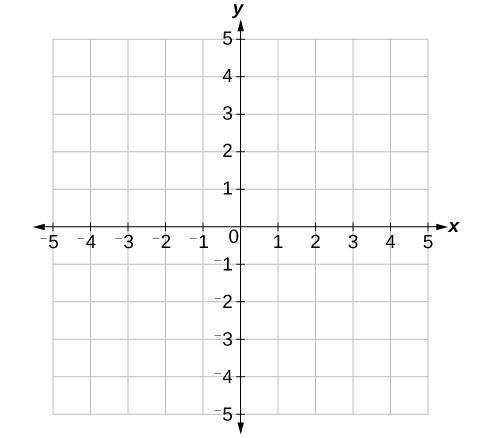
\includegraphics[width=0.75\textwidth]{CNX_CAT_Figure_02_01_201.jpg}
        \label{fig:enter-label}
    \end{figure}
    \hfill
    \newpage
    \item On the following axes, plot and clearly label the lines:
        \begin{enumerate}
            \item \(y = x\)
            \item \(y = -1\)
            \item \(y=-x\)
            \item \(x=3\)
        \end{enumerate}
    \begin{figure}[h]
        \centering
    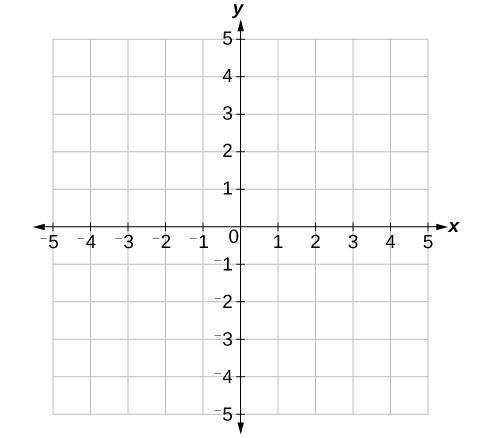
\includegraphics[width=0.75\textwidth]{CNX_CAT_Figure_02_01_201.jpg}
        \label{fig:enter-label}
    \end{figure}
    \hfill 
    \newpage
    \item Determine the prime factorisation of 4116.
    \vspace{8cm}
    \item The number 4356 is a square number. Prove that this is true and hence find its square root.
    \vfill
    \item A number which is neither prime nor equal to 1 is called what?
    \vspace{4cm}
    \newpage
    
    \noindent \textbf{Extension}
    
    \medskip
    
    The first and third digit, \(x\), of the 5-digit number
    \[
    x6x41
    \]
    are the same. The number is divisible by 9. What is the number?
    



    
    \newpage
    
 
\end{enumerate}






\newpage

\noindent \textbf{Topic Test 3: Fractions and Transformations}

\medskip

\hrule 

\medskip 

\begin{enumerate}
    \item Evaluate the following leaving your answers as either improper or proper fractions:
    \begin{enumerate}
        \item \( \frac{3}{7}+\frac{7}{9} \)
        \vspace{4cm}
        \item \( \frac{23}{24}-\frac{3}{8} \)
        \vspace{4cm}
        \item \( \frac{3}{10} \times \frac{5}{8} \)
        \vspace{4cm}
        \item \( \frac{2}{7} \div \frac{4}{5} \)
        \vspace{4cm}
    \end{enumerate}

\newpage

    \item Perform the following transformations on the yellow triangle:
    \begin{enumerate}
        \item Rotation by 180\(^\circ\) about the point \((1,0)\). Label it \(A\). \\
        \item Translation by the vector \(
		\begin{pmatrix}
        -2 \\
        -4 \\
		\end{pmatrix}
		\). Label it \(B\). \\
        \item Reflection in the \(y\)-axis. Label it \(C\).
    \end{enumerate}
    \begin{figure}[ht]
	\centering
	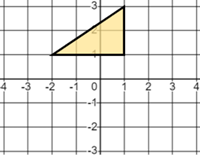
\includegraphics[width=0.75\textwidth]{Picture2.png}
    \end{figure}

\newpage

    \item Evaluate the following leaving your answers as mixed numbers:
    \begin{enumerate}
        \item \( 2\frac{1}{2} + \frac{3}{4} \)
        \vspace{4cm}
        \item \( 1\frac{5}{8} - 3\frac{4}{7} \)
        \vspace{4cm}
        \item \( 2\frac{1}{3} \times 3 \frac{3}{4} \)
        \vspace{4cm}
        \item \( 2\frac{5}{8} \div 1\frac{1}{6} \)
        \vspace{4cm}
    \end{enumerate}

\newpage


    \newpage
    \item Describe the following transformations as shown in the diagram:
    \begin{enumerate}
        \item \(A\) to \(C\) \\
        
        \underline{\hspace{13cm}} \\
        
        \underline{\hspace{13cm}} \\

        \item \(D\) to \(B\) \\
                
        \underline{\hspace{13cm}} \\
        
        \underline{\hspace{13cm}} \\
        \item \(C\) to \(B\) \\
                
        \underline{\hspace{13cm}} \\
        
        \underline{\hspace{13cm}} \\
    \end{enumerate}
    \begin{figure}[ht]
        \centering
        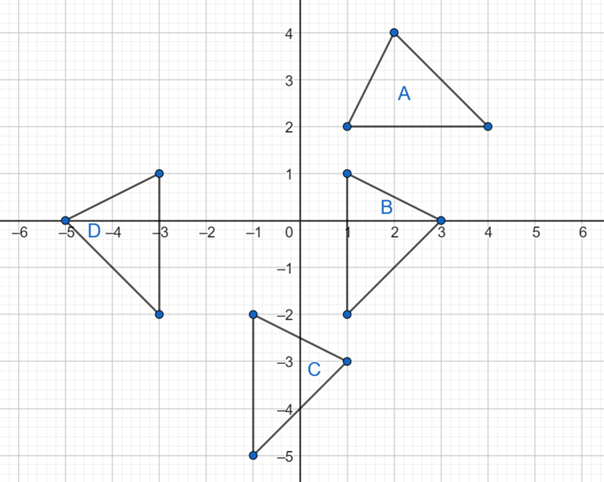
\includegraphics[width=0.75\textwidth]{Picture3.png}
        \label{fig:enter-label}
    \end{figure}

\end{enumerate}

\newpage

\noindent \textbf{Extension}

\begin{enumerate}
    \item Evaluate
    \[
    2 + \frac{1}{1+\frac{1}{4+\frac{1}{3}}}
    \]

    \vspace{8cm}

    \item Evaluate 
    \[
    2 \div ( 4 \div ( 6 \div ( 8 \div 10 ) ) )
    \]
\end{enumerate}

\newpage

\noindent \textbf{Topic Test 4: Algebra and Geometry}

\medskip

\hrule 

\medskip

\begin{enumerate}
    \item Simplify the following expressions:
    \begin{enumerate}
        \item \(4(2a+1)\)
        \vspace{2cm}
        \item \(b(b-3)\)
        \vspace{2cm}
        \item \(2c(5-2c)\)
        \vspace{2cm}
        \item \(-2d(d-5)\)
        \vspace{2cm}
        \item \(3x^2(2-6x)\)
        \vspace{2cm}
        \item \(x(3y-1)\)
        \vspace{2cm}
        \item \(-2z^2(x-y)\)
        \vspace{2cm}
        \item \(6x(x-3x^2+1)\)
        \vspace{2cm}
    \end{enumerate}

    \item A rectangle has one of its lengths 6cm longer than the other. The shorter length is denoted by \(x\).
    
    \begin{enumerate}
        \item Find and simplify an expression for the area of the rectangle.
        \vspace{3cm}
        \item Find and simplify an expression for the perimeter of the rectangle.
        \vspace{3cm}
    \end{enumerate}

    \item Simplify the following expression:
    \[
    3(1+4x) - 5(2+6x)
    \vspace{3cm}
    \]

    \item Consider the term \(-3x^7\)

    \begin{enumerate}
        \item What is the coefficient of this term?
        \vspace{2cm}
        \item What is the index of this term?
        \vspace{2cm}
        \item What is the variable of this term?
        \vspace{2cm}
    \end{enumerate}

    \item Find the unknown angle in each case below. You do \textbf{NOT} need to give reasons for your answers but should show your working.
    \begin{enumerate}
        \item \,
        \begin{figure}[h]
        \centering
            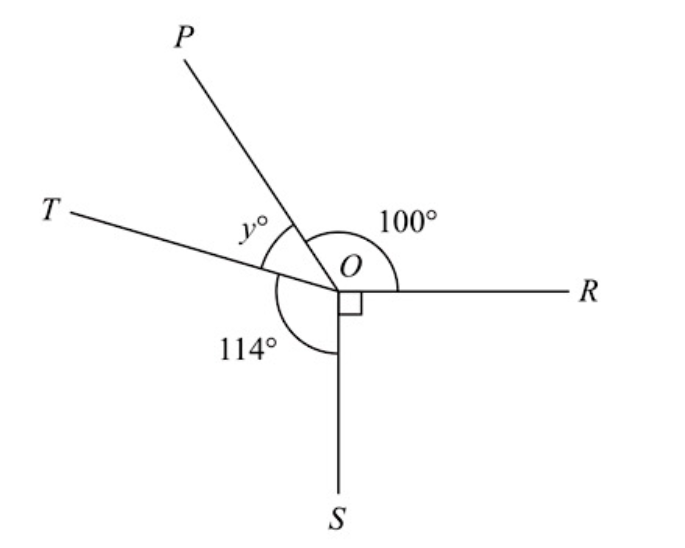
\includegraphics[width=0.5\textwidth]{Angles1.png}
        \end{figure}
        \item \,
        \begin{figure}[h]
        \centering
            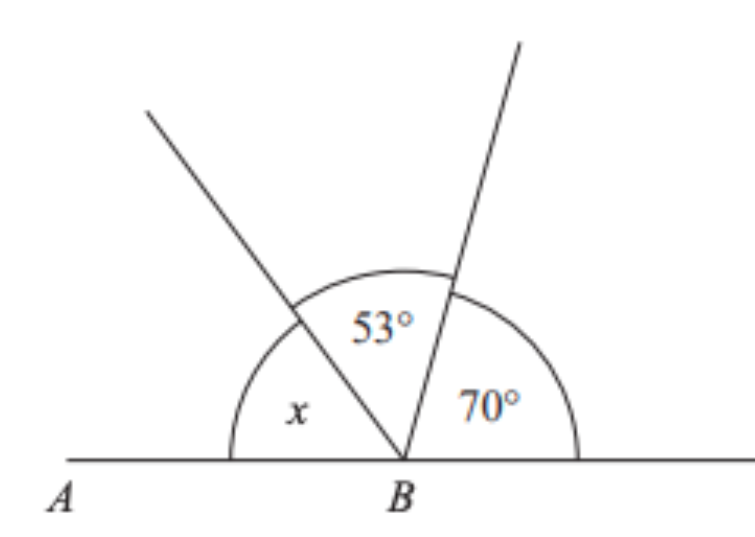
\includegraphics[width=0.4\textwidth]{Angles2.png}
        \end{figure}
        \vspace{2cm}
        \item \,
        \begin{figure}[h]
        \centering
            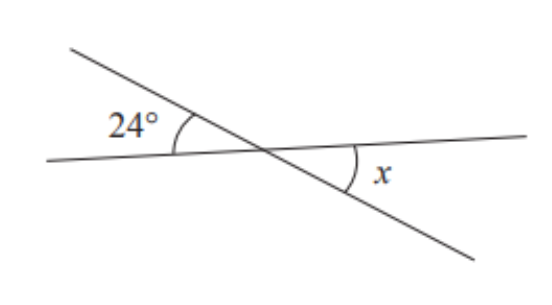
\includegraphics[width=0.4\textwidth]{Angles3.png}
        \end{figure}

        \newpage
        
        \item \,
        \begin{figure}[h]
        \centering
            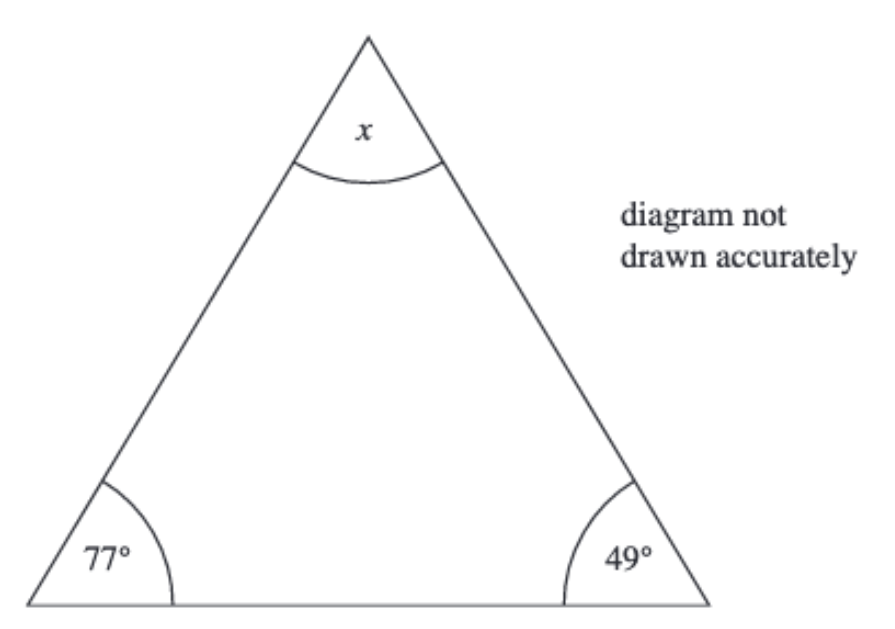
\includegraphics[width=0.5\textwidth]{Angles4.png}
        \end{figure}
        \vspace{3cm}
        \item \,
        \begin{figure}[h]
        \centering
            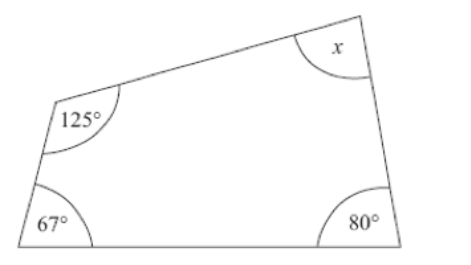
\includegraphics[width=0.5\textwidth]{Angles5.png}
        \end{figure}
    \end{enumerate}

    \newpage

    \item In each of the questions below, find the value of \(A\) by substituting the values for \(x\) and \(y\) into the given equation.
    \begin{enumerate}
        \item \(A = x-5  \text{ when } x=3\)
        \vspace{4cm}
        \item \(A = 3x + 1  \text{ when }x=2\)
        \vspace{4cm}
        \item \( A = 2x^2 - 1  \text{ when } x=-3 \)
        \vspace{4cm}
        \item \(A = 3x-2y \text{ when } x=-7, y = 5\)
        \vspace{4cm}
    \end{enumerate}

    \newpage

    \item In this question, you \textbf{MUST} give reasons for each stage of your working.
    \begin{enumerate}
        \item Find the angle \(DCB\).
        \item Find the angle \(x\).
        
        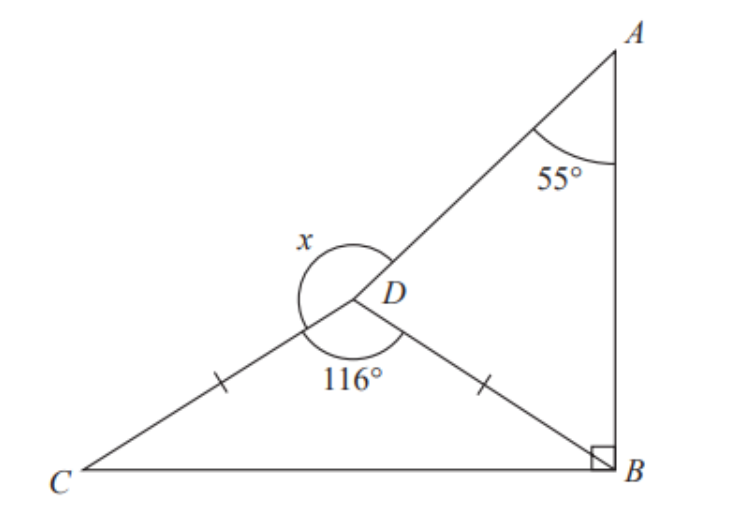
\includegraphics[width=0.5\textwidth]{Angles6}
    \end{enumerate}
    
\end{enumerate}

    \newpage
    
    \noindent \textbf{Extension}

    \begin{enumerate}
        \item In the diagram below, you are given that the lengths \(BC=CD\) and \(AB=AC\). The line \(CD\) cuts the angle \(ACB\) in half. What is the size of angle \(CDA\)?
    

    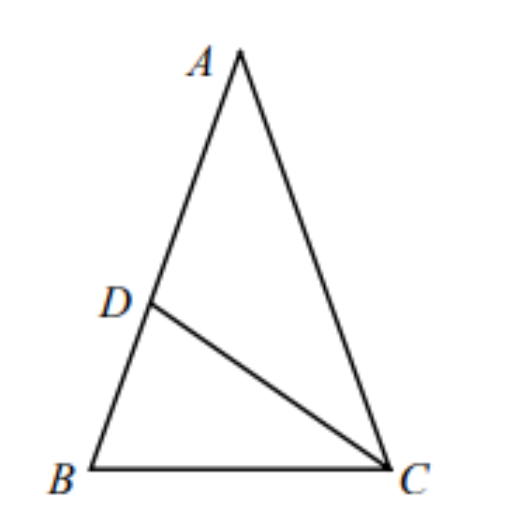
\includegraphics[width=0.3\textwidth]{Angles7.png}

    \vspace{5cm}

    \item Find the value of \(u\) when \(x=2\) if \(u\) is given by the equation
    \[
    u = \frac{-3^x}{4} \div \frac{7}{2x-1}
    \]

    \end{enumerate}


\newpage

\noindent \textbf{Topic Test 5: Decimal Arithmetic and Solving Equations}

\medskip

\hrule

\begin{enumerate}
    \item Evaluate the following:
    \begin{enumerate}
        \item \(32.1247 + 3.21247\)
        \vspace{4cm}
        \item \(0.0741 - 1.32\)
        \vspace{4cm}
        \item \(13.1 \times 3.69\)
        \vspace{4cm}
        \item \(0.144 \div 2.4\)
        \vspace{4cm}
    \end{enumerate}

    \newpage
    
    \item Solve the following equations. Leave your answers as improper or proper fractions as necessary.
    \begin{enumerate}
        \item \(2a+4=10\)
        \vspace{4cm}
        \item \(2(b+3)=6\)
        \vspace{4cm}
        \item \(8-7c=-6\)
        \vspace{4cm}
        \item \(3(2-d)=24\)
        \newpage
        \item \(5w-5=2=3w\)
        \vspace{4cm}
        \item \(4(2x-3)-3(x+2) = 2x\)
        \vspace{4cm}
        \item \(\frac{9y-12}{5}=3\)
        \vspace{4cm}
        \item \(4-\frac{z-2}{2}=z+\frac{1-2z}{3}\)
    \end{enumerate}

    \newpage

    \item The result of doubling a number and adding 17 is the same as trebling it (multiplying by 3) and adding 4. What is the number?

    \vspace{8cm}

    \item A cup of tea costs 10p less than a coffee and a hot chocolate costs 20p more than a coffee. The cost of three coffees, five cups of tea and two cups of hot chocolate is £26.70.

    \begin{enumerate}
        \item Form an equation with \(x\) representing the price of a coffee.
        \item Solve your equation to and hence determine the price of each beverage.
    \end{enumerate}
\end{enumerate}

\newpage

\noindent \textbf{Extension}

\medskip

\begin{enumerate}
    \item Solve the following equation:
    \[
    8.9(x-3.5)-4.2(3x+2.3)=4.7x+1.19
    \]
    \vspace{7cm}
    \item Solve the following equation:
    \[
    \frac{1}{2}(1-x)-\frac{1}{3}(2+x)+\frac{1}{4}(3-x)=1
    \]
    
\end{enumerate}



\end{document}
